\title{Acceleration of plague outbreaks in the second pandemic}

\author{David J.\,D.\ Earn$^{a,b,c}$, 
Junling Ma$^{f}$, 
Hendrik N.\ Poinar$^{b,c,d,e}$,\\
Jonathan Dushoff$^{a,b,c}$,
and Benjamin M.\ Bolker$^{a,b,c}$\\
\href{mailto:earn@math.mcmaster.ca}{\tt earn@math.mcmaster.ca}\\
\small $^a$Department of Mathematics \& Statistics, $^b$Department of Biology, \\
\small $^c$Michael G.\ deGroote Institute for Infectious Disease Research,\\
\small $^d$McMaster Ancient DNA Centre, Department of Anthropology,\\
\small and $^e$Department of Biochemistry,\\
\small McMaster University, 1280 Main Street West, Hamilton, ON, L8S 4K1, Canada;\\
\small $^f$Department of Mathematics \& Statistics, University of Victoria, Victoria, BC, Canada}

\begin{document}

\linenumbers

\maketitle

%%\begin{abstract}
{\bfseries
\noindent
Historical records reveal the temporal patterns of a sequence of plague epidemics in London, England, from the 14th to 17th centuries.  Analysis of these records shows for the first time that later epidemics spread significantly faster (``accelerated'').  Between the Black Death of 1348 and the later epidemics that culminated with the Great Plague of 1665, we estimate that the epidemic growth rate increased \foldval.
%%[\rdiffest $\times$, 95\% CI: \rdifflwr $\times$ to \rdiffupr $\times$].  
%%The cause of this change is unknown; despite rapid recent advances in paleogenomics, it is hard to confirm or reject the possibility of functional evolutionary changes in circulating strains of the plague bacterium \ypestis over this time period.
Currently available data do not provide enough information to infer the mode of plague transmission in any given epidemic; nevertheless, order-of-magnitude estimates of epidemic parameters suggest that the observed slow growth rates in the 14th century are inconsistent with direct (pneumonic) transmission.  
We discuss the potential roles of demographic and ecological factors, such as climate change or human or rat population density, in driving the observed acceleration.
}  
%%\end{abstract}

\bigskip

\leftline{plague $|$ London $|$ epidemic growth rate $|$ reproduction number $|$ SARS-CoV-2 $|$ COVID-19}

\bigbreak

\noindent\fbox{\parbox{0.98\textwidth}{{\bfseries Significance Statement:} 

Epidemics of plague devastated Europe's population throughout the Medieval and Renaissance periods.  Genetic studies of small numbers of skeletal remains indicate that the causative agent of all these epidemics was the bacterium \emph{Yersinia pestis}, but such analyses cannot identify overall patterns of transmission dynamics.
Analysis of thousands of archival records from London, England, reveal that plague epidemics spread much faster in the 17th century than in the 14th century.}}

\bigbreak

\dropcap{P}lague epidemics have afflicted human populations since at least the 6th century \cite{McNe76,Wagn+14}.  These events have had dramatic and long-lasting effects on human demography and behaviour, especially those outbreaks associated with the ``second pandemic'' (14th--19th centuries) in Europe and Asia \cite{Pepy1669,Lath85,Defo1722,McNe76}, and have inspired many
theoretical studies of the ecology and evolution of infectious disease \cite{KermMcKe27,AndeMay91,KeelGill00,Baca12,Silv16,LewnTown16,Yue+16,Dean+18}.
We are now in the third pandemic (Modern Plague), with outbreaks continuing to occur in some parts of the world \cite{PerrFeth97,Neer+10,WHO10,ECDC17,Robe17}. Plague also remains a source of concern due to the bioterror potential of the causative agent, \emph{Yersinia~pestis} \cite{Ligo06,CDCplagueEmergencyFAQ}. 

Recent advances in paleogenomics have definitively established that historical plague pandemics were caused by \ypestis
 \cite{Bos+11,Bene11}, as proposed in the 19th century after Yersin discovered the bacterium's link to bubonic plague \cite{Butl14}.
 Researchers have reconstructed the evolutionary history of plague and other pathogens by sequencing and reconstructing nearly complete pathogen genomes from persistent DNA fragments \cite{Schu+11, Bos+11,Deva+14}.
 The strain isolated from victims of the Black Death (London 1348) is  remarkably similar to extant human strains (Modern Plague): 
the core genomes\footnote{The core genome is about 80\% of the full genome, shared between all sequenced strains of \ypestis.} of these strains are $\approx 99.99\%$ similar \cite{Bos+11}, which makes it challenging to 
identify important evolutionary or ecological patterns
from genomic investigations alone.  Here, we complement genetic studies by exploring more traditional (historical, demographic, and epidemiological) sources of information
from a 300-year span of plague outbreaks in the same location (London), revealing a striking change in plague transmission dynamics over the course of the Renaissance period, namely a \foldval increase in the initial growth rate of outbreaks.

We quantify this change without making any assumptions about the underlying transmission processes, exploiting methodology that we have developed previously for this purpose \cite{Ma+14}.  We then consider how this inference can contribute to the debate concerning whether plague transmission was primarily indirect (via rat fleas) or direct (pneumonic human-to-human).  We argue that strictly pneumonic transmission in the 14th century is implausible, but that beyond this the best that can be done at present is to highlight the biological complexities and uncertainties that limit the potential for further inferences.

\mysection{Data}

The city of London, England, is unusual in the extent to which patterns of death and disease can be reconstructed from extant documents. We have analyzed three sources of data (\cref{F:plot3sources}):
\begin{description}
\item[London Bills of Mortality] The London Bills of Mortality \cite{Crei65,Tien+11} (LBoM) provide weekly counts of deaths by cause during each of the known plague epidemics in the 16th and 17th centuries.  The LBoM thus give us information specifically about mortality attributable to plague for each epidemic, which we will use as a proxy for plague incidence \cite{KermMcKe27,Ma+14}.  When available, the LBoM are our most reliable records (except for the epidemic of 1593; see \supp).
\item[Parish registers] After 1538 \cite[p.\,54]{Slac90}\cite{Wall04}, London parish registers provide information on mortality.
%%, although these are not categorized by cause. 
We use weekly counts of deaths published online by Cummins, which are estimated to cover 80\% of total deaths \cite{Cumm+16}. During plague epidemics, most deaths were likely due to plague; we also adjust for non-plague mortality by estimating a baseline death rate from the years before and after an epidemic (see \Methodslink).
\hypertarget{mainsec:Data.wills}{}
\item[Wills and testaments] Before 1538, no direct tabulations of mortality for London are available. However, we do have detailed information on last wills and testaments, which can be used as proxies for mortality \cite{Slac90}. In particular, we have digitized and tabulated daily counts of wills recorded in the Court of Husting \cite{Shar1889} for the 14th century; these give us data for the plague epidemics of 1348, 1361, 1368 and 1375 (monthly counts for three of these epidemics were previously published by Cohn \cite{Cohn03}). We use online data from the Prerogative Court of Canterbury (PCC) \cite{Archives2018} 
for the plague epidemics of the 16th and 17th century.  Plague epidemics in London are mentioned in historical documents from the 15th century \cite[Ch.\,IV]{Crei65}, but during this period wills recorded in the Courts of Husting and Canterbury were too sparse to enable identification of epidemics.

Two dates are associated with each will: the date on which it was written, and the date on which it was probated (\ie accepted by the court after the death of the testator). Traditionally, demographers have used annual counts of wills by probate date, as testators are known to have died by these dates. While this approach works well for inferring long-term trends in annual mortality, probate dates are inappropriate for reconstructing detailed time series of mortality over short time scales, as there is a variable and irregular lag between the (unknown) date of the death and the probate date; most of the wills associated with 14th century epidemics were probated several months after they were written \cite{Bush19} (see \cref{F:willsVSprobates}).
  
Instead, we use the counts of wills \emph{written} in a given time interval
as a proxy for plague incidence. The date on which a will was written may precede the testator's death by a long period, but during severe epidemics will dates were likely to have been correlated with the fear of infection (and hence with disease incidence), just as internet searches for influenza symptoms can predict 21st century epidemic patterns \cite{Gins+09}.

When using wills as proxies for mortality or incidence, we must keep in mind that: 1) a much smaller proportion of the population is sampled (the will counts in \cref{F:plot3sources} are about 10 times smaller than the counts based on parish registers); 2) the subpopulation of individuals who wrote wills is strongly biased towards merchants and others who owned property (primarily males).
\end{description}

For the period since 1540, the existence of multiple sources allows us to cross-check results---in particular, to test our assertion that aggregated counts of wills by date written are an adequate proxy for mortality rates---and avoid relying on any questionable or poorly sampled segments of data \cite{RoosCurt18} (see \supp). In 1563 and 1593, the number of PCC wills is too small to extract a signal from the noise, but the data for the later three outbreaks verify that the numbers of wills written follow the plague epidemic patterns evident in the mortality records (\cref{F:timeseries}). Based on cross-correlation analysis and differences between epidemic peak times, will counts appear to have lagged mortality recorded in parish registers and LBoM by approximately 3--5 weeks; our inferences about epidemic growth rates appear to be robust to this lag (see \supp). 

The LBoM indicate that there were 18 other plague epidemics in London between 1563 and 1666; these were all of much smaller magnitude and are discussed only in \supp.  No plague epidemics have occurred in London since the end of the Great Plague in 1666: a total of 77 deaths from plague are recorded in the LBoM after 1666, never more than 5 in a single week.  The last plague deaths recorded in the LBoM occurred during the week of 6 May 1679.

%
\newcommand{\pixht}{0.3\textheight}
\begin{figure}
\begin{center}
\mbox{
\hspace{1.2cm}
\includegraphics[height=\pixht]{images/WillExample1644_page86_1.pdf}
%% \includegraphics[height=\pixht]{WillExample1644_page86_1.eps}
\hspace{0.4cm}
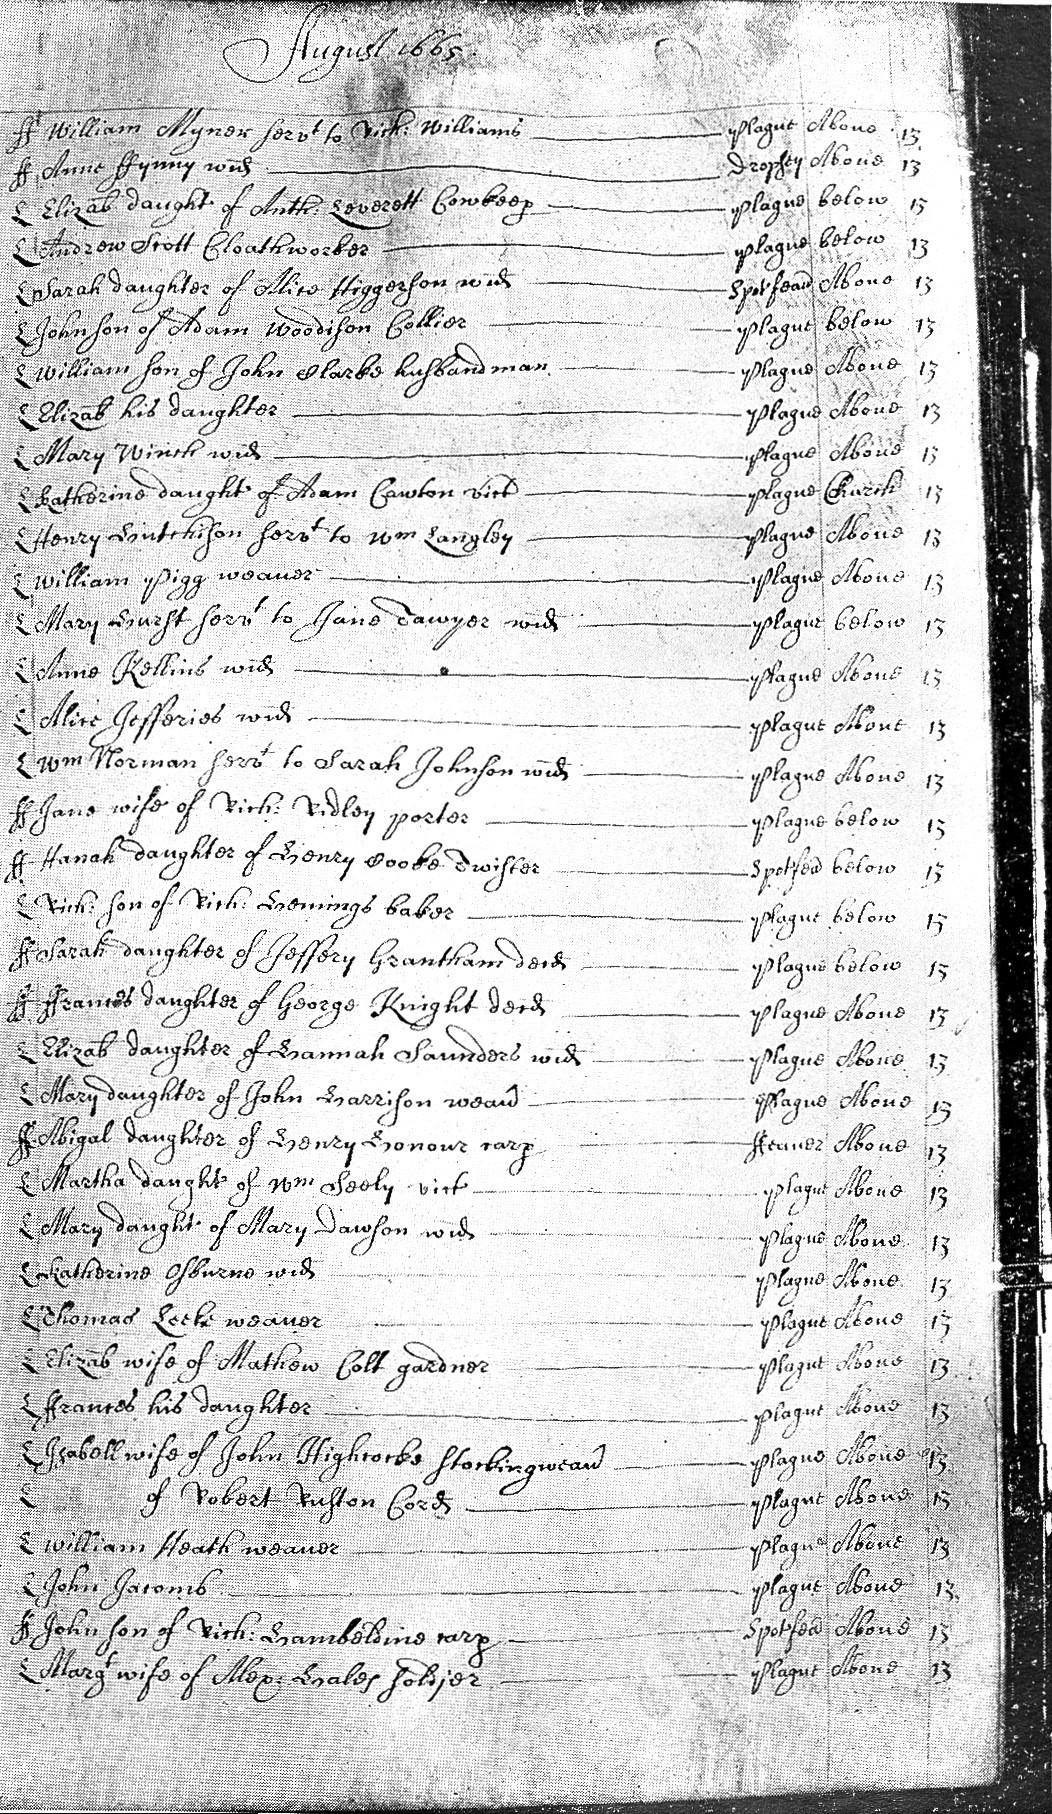
\includegraphics[height=\pixht]{images/cripplegate_wellcome_parish.jpg}
%% 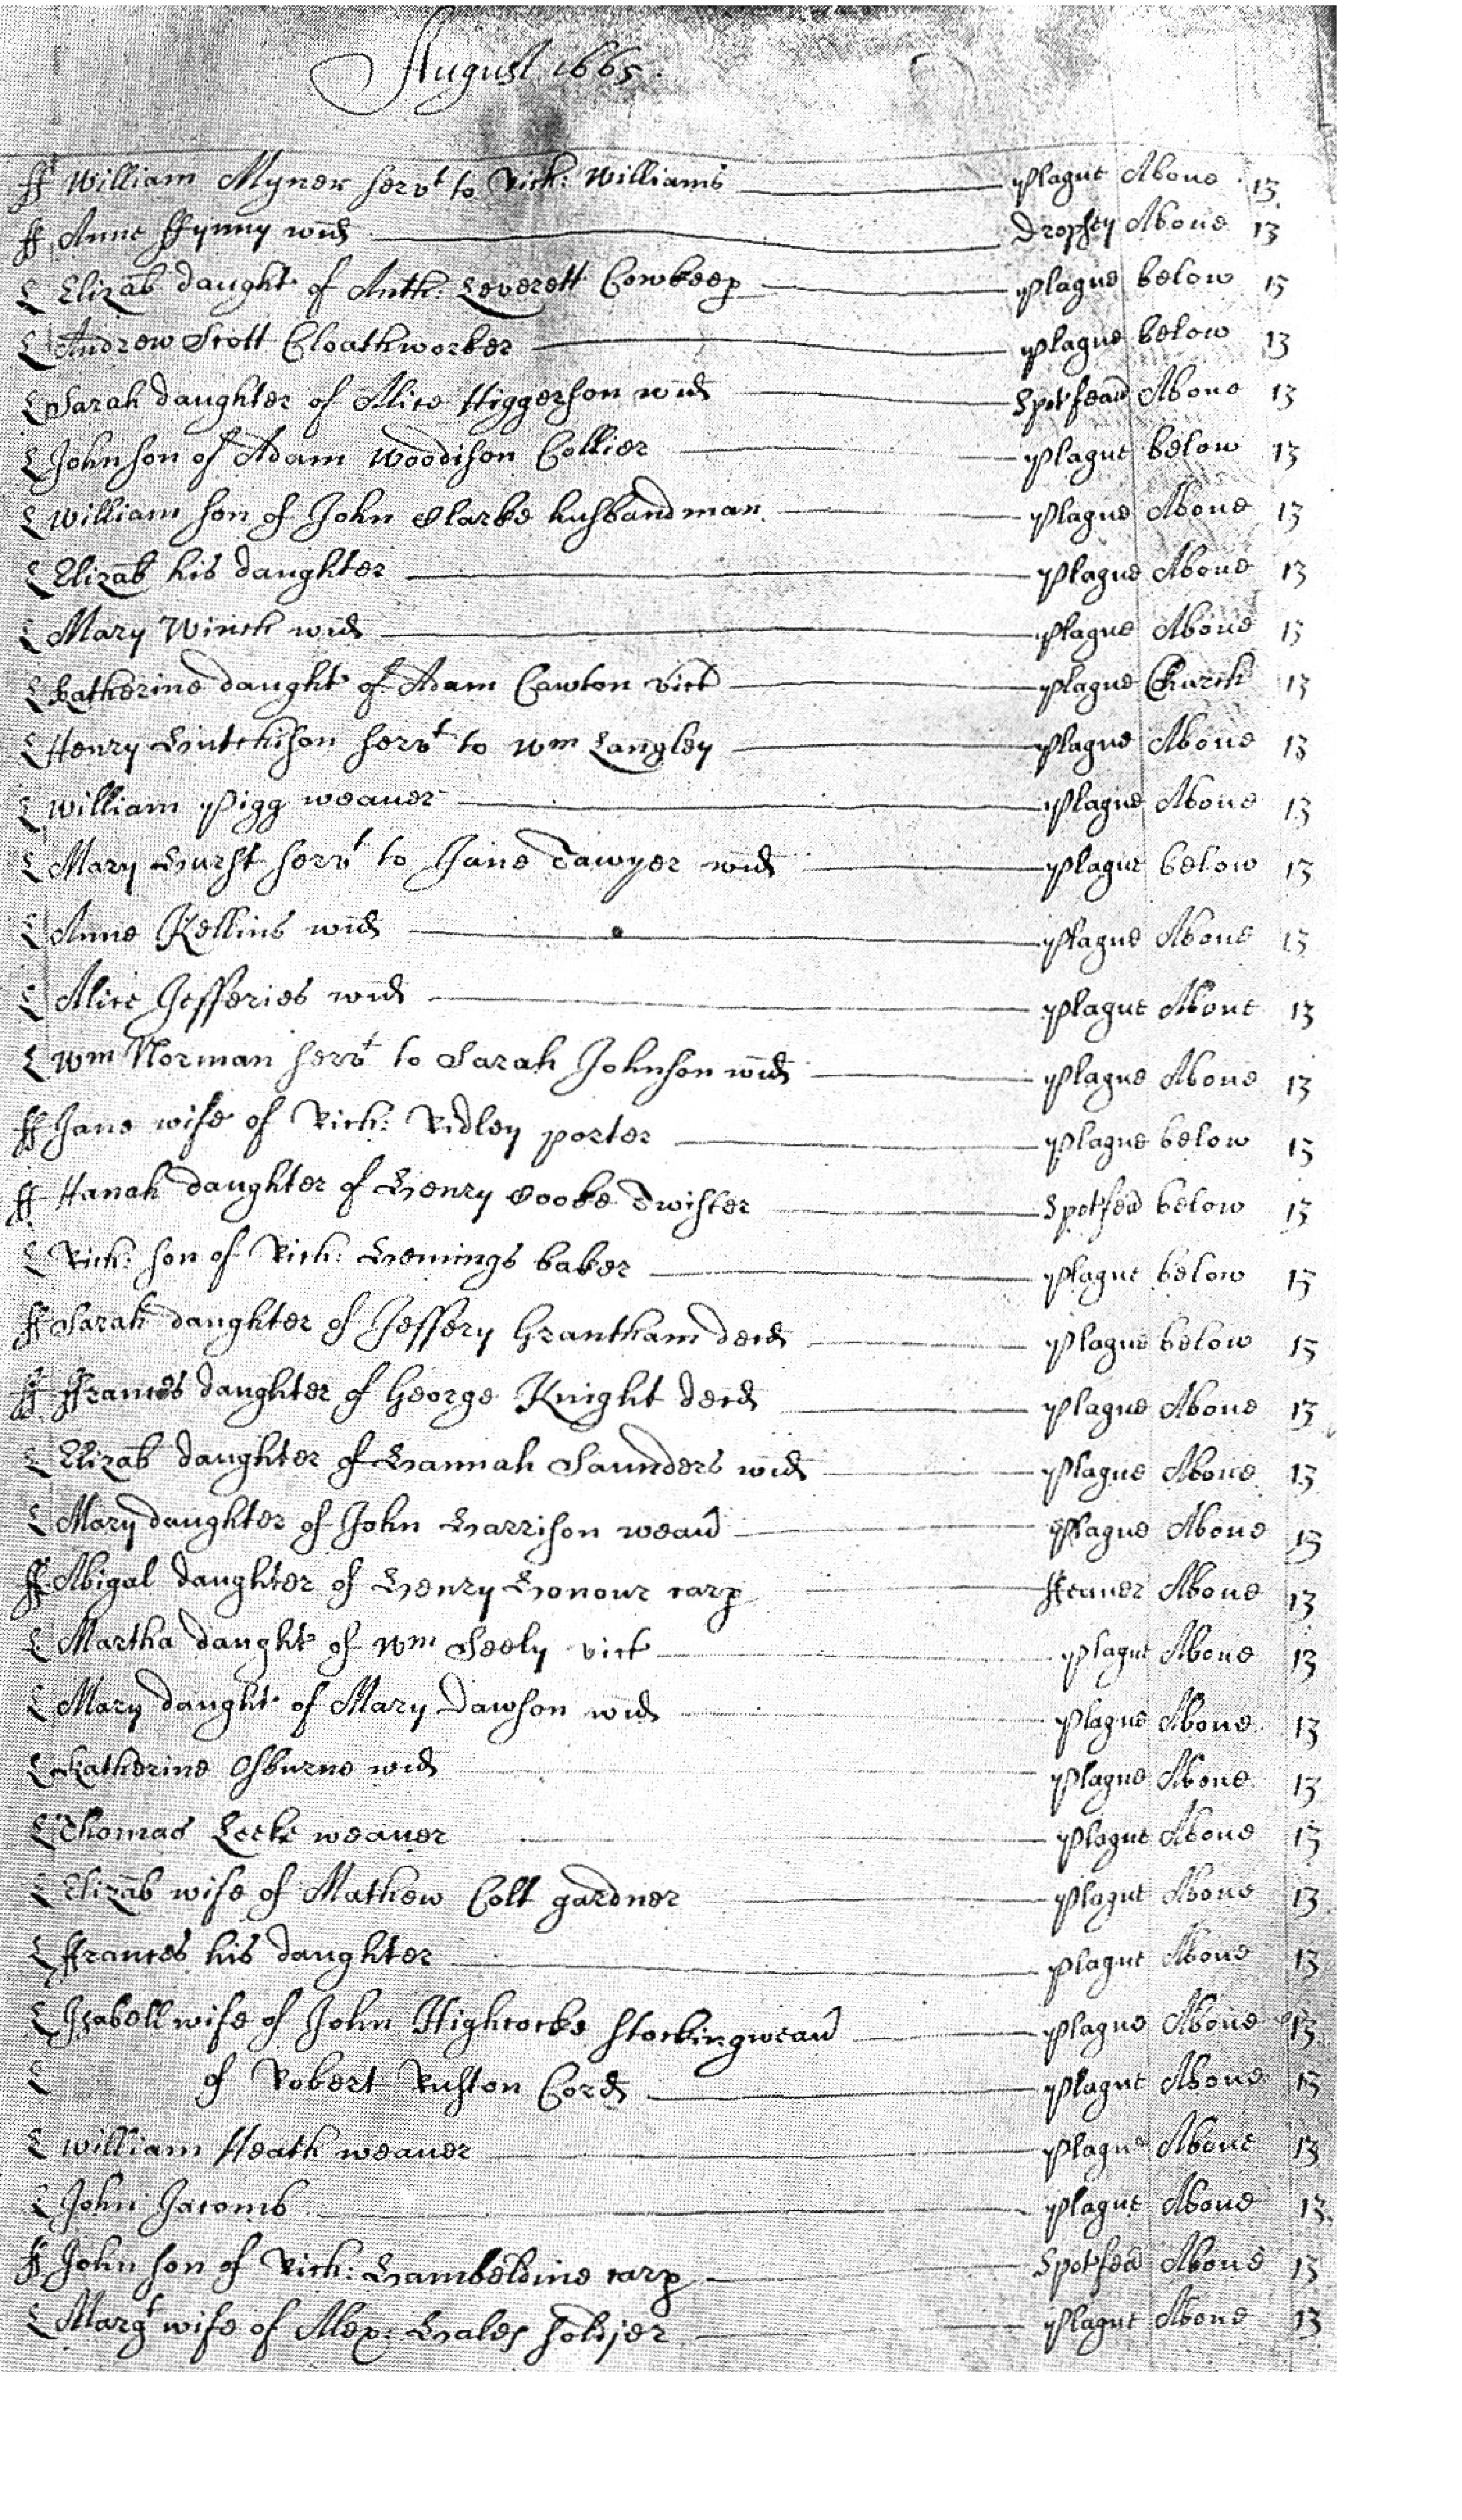
\includegraphics[height=\pixht]{cripplegate_wellcome_parish.eps}
\hspace{0.4cm}
\includegraphics[height=\pixht]{images/bill1665adjust.pdf}
%% \includegraphics[height=\pixht]{bill1665adjust.eps}
}
\\ \vspace{0.5cm}
\includegraphics[width=\textwidth]{analysis/plots/plot_allsources.pdf}
%% \includegraphics[width=\textwidth]{plot_allsources.eps}
\end{center}
\vspace{-0.5cm}
\caption[]{
  \emph{Top left:} Part of a will proved in the Prerogative Court of Canterbury (PCC), dated 18 December 1644 \cite{Archives2018}.
  \emph{Top centre:} A parish register page from St Giles without Cripplegate, August 1665 \cite[courtesy of the Wellcome Collection: \url{https://wellcomecollection.org/works/uutd7scc}]{Bell24}.
  \emph{Top right:} One of the London Bills of Mortality (LBoM), for the week beginning 26 September 1665 (photo by Claire Lees).
\emph{Bottom:}
Mortality in London, England, 1340--1380 and 1540--1680, aggregated 4-weekly, plotted on a log scale.  The three distinct sources of data (see \cref{tab:datasources}) are: 
last wills and testaments of Londoners whose wills were probated in the the Court of Husting (14th c.{}) or the PCC (16th-17th c.{}),
weekly aggregations of burials listed in extant parish registers \cite{Slac90}, 
and weekly plague deaths listed in the LBoM \cite{Crei65}.
Major plague years are highlighted in yellow.  Aside from these and various minor plague years, there are notably unusual patterns during an epidemic of ``sweating sickness'' in 1551 \cite[p.\,70]{Slac90}, the ``influenza'' epidemic of 1557--9 \cite[p.\,70]{Slac90} (which coincided with the end of the reign of ``Bloody'' Mary~I and the ascension of Elizabeth~I in 1558 [indicated by a crown icon]), and the absence of a monarch during the Interregnum from 30 January 1649 to 29 May 1660.
}
\label{F:plot3sources}
\end{figure}
%

\mysection{Approach}

\paragraph{Estimation of epidemic growth rates}

While our collection of high-resolution mortality time series during plague epidemics allows us to estimate epidemic growth rates, we are constrained by the limitations of our data---the time series for each epidemic are short and noisy, especially during the 14th century (\eg the epidemics of 1368 and 1375 peaked at a total of 5 wills written per week). Thus we chose to use simple phenomenological models with a small number of parameters that can be fitted to short time series (starting size, growth rate, and total size: see \Methodslink), and do not attempt to separate different sources of variability or estimate the influence of various mechanistic processes (King \etal's exhortation to use epidemic models that separate process from observation noise \cite{King+2015} applies primarily to forecasting, which we are not attempting).
Furthermore, we primarily consider the initial growth rate $r$, which---unlike the basic reproduction number $\rzero$---can be estimated reliably from mortality data alone without any knowledge of the disease characteristics or natural history \cite{Ma+14}.

We estimate the epidemic growth rate for each epidemic as the maximum likelihood estimate of the initial growth rate of a logistic function fitted to the cumulative death curve (using first differences to avoid over-confidence; see \Methodslink\ for more detail), along with likelihood profile confidence intervals (CIs). To summarize the overall difference between epochs, we then use the estimates for each epidemic as observations in a linear mixed model including fixed effects of epoch (``early''/14th c.\ \emph{vs.}\ ``late''/16th-17th c.{}) and data source, and a random effect of outbreak year (see \hyperlink{outbreak.year}{below}), where each estimate was weighted by its certainty.

Finally, to robustly quantify the statistical significance of the difference between epochs, we ran a permutation test. We computed the null distribution of the between-epoch difference in growth rate by scrambling the estimates and associated CIs randomly across epochs. For each of the 126 possible permutations, we refitted the mixed model and extracted the estimated among-epoch difference in growth rate.

\paragraph{Estimating $\rzero$ and attack rate}

Our analysis focuses on the epidemic growth rate $r$, rather than the more commonly investigated basic reproduction number $\rzero$ (the expected number of secondary cases caused by a primary case in a completely susceptible population \cite{AndeMay91}), because estimates of $\rzero$ depend on information about the life history of the pathogen as well as on the epidemic curve itself \cite{WallLips07}. However, if we can estimate $\rzero$ then we can predict epidemic outcomes that we are unable to predict from $r$ alone; then, by comparing observed with theoretical outcomes under different scenarios, we can make inferences about modes of transmission.

In particular, if the host population is homogeneously mixed, we can use $\rzero$ to estimate the expected final size $Z$ (the proportion of the population infected by the end of an epidemic, also called the \emph{attack rate}) \cite{KermMcKe27,MaEarn06}. The \emph{observed attack rate} based on mortality records depends in turn on the fraction of infected individuals who die from disease. We can thus compare theoretical expectations of observed attack rates under different transmission modes with historical information about observed attack rates (see \hyperlink{implications}{Implications}).

We can use the distribution of the generation interval (the times elapsed between the moment a host is infected and the times at which they infect others) to compute $\rzero$ from $r$ \cite{WallLips07}. If we know only the \emph{mean} generation interval $\gentime$, we can still approximate $\rzero \approx r \gentime +1$, by assuming that the generation intervals are exponentially distributed; this approximation underestimates $\rzero$ in the typical case where the generation interval distribution is less variable than an exponential distribution with the same mean.

Beyond the information on generation interval that we use to derive $\rzero$ from $r$, the observed attack rate depends on additional characteristics of an epidemic. If the population does not mix homogeneously, the final size will typically decrease (\eg \cite[Fig.\,6]{Roll+15}). Since the \emph{case fatality proportion} (CFP, the proportion of plague cases who die) is not 100\%, the observed attack rate is less than the final size. Observed attack rates also decrease if some individuals are infected without showing symptoms (asymptomatic infections) \cite{Mars+67}, or without symptoms identified as plague (sub-clinical infections). Finally, the observed attack rate depends on the initial proportion of the population susceptible, which will be lower if some individuals have previously acquired immunity after previously non-fatal plague infections. 

We can use independent estimates of the generation interval to estimate $\rzero$ (and hence the theoretical attack rate) for London epidemics under different transmission modes.  Given the limited information that we have, we consider the additional (extreme) assumptions that \hypertarget{4assumptions}{} (1) the population was homogeneously mixed; (2) the population was initially 100\% susceptible; (3) there were no asymptomatic infections; and (4) all infected individuals died (\ie the CFP was 100\%). All of these assumptions increase the observed attack rate (as detected from wills or deaths), so we can calculate an upper bound on the total mortality we would expect to observe in an epidemic with a particular transmission mode.

\mysectionsamepage{Results}

The fitted models do as good a job as one could hope for in capturing the initial patterns of epidemic growth evident in the noisy will counts, and agree very well with the patterns of growth in the mortality time series that are available in the later epoch (\cref{F:timeseries}).

The growth rates for the 14th century epidemics are lower than those for the 16th-17th centuries (\cref{F:combdata}); they may also be more variable than in the later period, although some of the appearance of variability is due to larger uncertainties (presumably due to the relatively poor sampling in the early epoch). The mixed model quantifies the dramatic increase in growth rate (``acceleration'') of epidemics between epochs.
The growth rates increased \foldval in the late \emph{vs.}\ early epochs: $r$ increased \rdiffest $\times$ [95\% CI $(\rdifflwr\times, \rdiffupr\times)$] (see \Methodslink). The permutation test results support the statistical significance of this difference; the observed order of outbreaks yields the most extreme difference in growth rates out of all \nperm\ possible orderings, giving a two-tailed $p$-value of $\permfrac=\permpval$.


%
%%\begin{figure}[h!]
\begin{figure}
\begin{center}
\includegraphics[width=\textwidth]{analysis/plots/timeseries.pdf}
%% \includegraphics[width=\textwidth]{timeseries.eps}
\end{center}
\caption[]{Observed time series (points) and \hyperlink{phenmod}{phenomenological model} fits (lines; see \Methodslink) that yield the estimated growth rates (listed in \cref{tab:params} and plotted in \cref{F:combdata}).  The data sources (\cref{tab:datasources}) are described in the main text and the caption to \cref{F:plot3sources}.  For visual comparison, wills were aggregated weekly to match the frequency of mortality observations (fits to wills were based on the original daily counts).
  \cref{F:plotwills14c,F:plot3sourcesmajors} display the data during the major plague epidemics on linear rather than logarithmic scales.
  Vertical dashed lines show 1 April, 1 July, and 1 October of each year.
  In 14th c. data (top row), zero-count weeks are shown along the bottom edge of the graph.
}
\label{F:timeseries}
\end{figure}
%

%
%%\begin{figure}[h!]
\begin{figure}
\begin{center} 
\includegraphics[width=6.5in]{analysis/plots/combdata.pdf} 
%% \includegraphics[width=6.5in]{combdata.eps} 
\end{center} \caption[Estimated initial growth rates]{Estimated initial growth rates ($r$) and 95\% profile CIs on a logarithmic scale, for each of the epidemics shown in \cref{F:timeseries}.  Center panels show mixed-model estimates (see \Methodslink) of overall average growth rate for each epoch (early:\ 14th c.\ \emph{vs.}\ late:\ 16th-17th c.{})\ and data source.  To aid interpretation, the additional vertical scales show the implied intrinsic reproductive number ($\rzerop$) and epidemic final size ($\Zp$) under the assumption that the generation interval distribution \cite{WallLips07} was the same as that estimated from 20th century pneumonic plague epidemics \cite{GaniLeac04}. All estimates and CIs are listed in \cref{tab:params} (which also lists the associated doubling times).}
\label{F:combdata}
\end{figure}
%

\begin{table}[h!] 
  \caption[Estimated $r$ and $1/r$]{Maximum likelihood estimates (MLEs) of the initial exponential growth rate ($r$) and doubling time ($(\log2)/r$) with their 95\% confidence intervals (CIs), obtained from the time series shown in \cref{F:timeseries} (see \Methodslink).  The goodness of fit measure ($R^2$) is the proportional reduction in the mean squared error, \ie $1-d^2/\sigma^2$ where $d^2$ is the model mean squared error and $\sigma^2$ is the (population) variance of the data; predictions and observations are aggregated to weekly before computing the $R^2$ for wills, for consistency among data sources. The implied basic reproduction numbers ($\rzerop$) and attack rates ($\Zp$), assuming the generation interval distribution for Modern pneumonic plague \cite{GaniLeac04}, are also shown.
All MLEs and associated CIs are shown in \cref{F:combdata}.
}
\begin{center}
  \footnotesize
  %%\rowcolors{2}{white}{verylightgray}
  \rowcolors{2}{white}{gray}
  \input{analysis/tables/params.tex}

\end{center}
\label{tab:params}
\end{table}

\FloatBarrier
\mysection{Discussion}

Plague epidemics in London appear to have been faster in the 16th-17th centuries than in the 14th. Our analysis shows that this difference is very likely real, rather than driven by changes in the types of documentary evidence that are available; in particular, we have shown that inferences from will counts are consistent with those from death counts when both are available, in the 17th century.

Why the later plague epidemics were faster than the earlier ones is not clear.  Nevertheless, to provide some context, we consider below a number of mechanisms that \emph{could} have contributed to increases in epidemic growth rates.  We then consider what our estimated epidemic growth rates suggest about the mode of transmission during the various London plague epidemics.

\subsection*{Possible causes of acceleration}

What factors could have caused plague epidemics in London in the 16th and 17th centuries to accelerate relative to the earlier plagues in the 14th century?

\paragraph{Pathogen or host evolution}

Faster growth could be a consequence of the pathogen evolving to infect hosts more effectively, or to remain infectious for longer.  However, such evolution may be challenging to demonstrate, particularly in light of the strong genetic similarity between the Second Pandemic and Modern Plague strains \cite{Bos+11}. Evolution of host resistance has also been suggested as a cause of changes in plague dynamics \cite{LewnTown16}, though we have no particular mechanisms in mind for how the evolution of resistance over the course of centuries could accelerate epidemics.

\paragraph{Shifts in transmission mode}

Modes of transmission may have differed between epochs, which could account for differences in epidemic growth rates.  The reservoir host of \ypestis in London was rat populations where it was primarily spread by flea vectors such as {{\em X.~cheopis}} \cite[p.\,54]{PerrFeth97}. This transmission mode gives rise to bubonic plague in humans, as a consequence of zoonotic spillover; epidemic growth rate is driven by spread among rats and fleas, with human infection and mortality as a secondary consequence. In contrast, when \ypestis infection in humans spreads to  the lungs, it gives rise to pneumonic plague, which can then spread directly from human to human like other severe respiratory infections.
It has also been more recently hypothesized that human ectoparasites (including lice and human fleas) could have supported indirect plague transmission without involving rats \cite{Dean+18,Laro+18}. 

Pneumonic plague probably has shorter generation intervals than bubonic plague \cite{GaniLeac04,LaPerriere+2009}, and is often thought to spread much faster at the population level \cite{GaniLeac04}; one \emph{potential} explanation for our observations is that 14th century epidemics were primarily bubonically transmitted while 16th-17th century epidemics were primarily pneumonic.  With currently available data, we are unable to confirm or reject this hypothesis, but we consider below whether any inferences about transmission mode can be made at present.

\paragraph{Ecological and demographic changes}

The complete multi-species ecology of \ypestis is extremely complicated \cite{DubyYesz16}.  We focus on humans because the only data available for the epochs studied here concern humans, and not on the rest of the ecological community supporting \ypestis.  Human population size and population density in London increased enormously from the 14th to 17th centuries \cite{Finl81,FinlShea86,Kryl11} (\cref{tab:pop,F:london_pop}), and density increases were exacerbated in the 17th century by the isolation of the sick and their contacts in pest houses [A.~Carmichael, \emph{pers.\ comm.}].  Since bubonic plague epidemics are driven by spillover from rat-flea epidemics, human population density would only have a direct effect on the speed of pneumonic epidemics.  However, changes in human population (and living conditions) almost certainly affect rat, and flea, density \cite{McCo03}.  In addition, higher rat densities make it more likely that fleas departing dying rats end up on susceptible rat hosts.  The magnitudes of these effects are extremely difficult to estimate, but in \supp we explore them in a (crude) quantitative manner, without attempting to model the truly complex population dynamics that occur even during a single epidemic \cite{KeelGill00b,LaPerriere+2009}.

\paragraph{Environmental change}

The external environment represents the third side of the host-parasite-environment ``disease triangle'' \cite{Scho07}.  Northern European climates changed significantly between the 14th and 16th--17th centuries (the coldest period of the ``Little Ice Age'' occurred in the 17th century \cite{Matt39} \cite[Figure 1]{Jone+13}).  Furthermore, late-epoch epidemics occurred later in the calendar year, and hence in different seasons (\cref{F:timeseries}).  A variety of studies link climate (\eg overall wetness/dryness) or weather (\eg annual precipitation or temperature) to plague incidence or transmission \cite{Cava71,Xu+11,Xu+14,Pham+09,YueLee18,BenA+10,Scho+11}.  Climatic changes may have been responsible for the changes in plague epidemics in London between 1348 and 1666, but it is challenging to make reliable inferences due to the lack of consensus about climate and weather variations in Medieval/Renaissance Europe \cite{Nesj+08}.

\hypertarget{implications}{}
\subsection*{Implications of growth rate estimates for transmission mode}
\label{sec:implications}

One might hope to exploit ancient DNA \cite{Bos+11,Wagn+14} to identify the transmission mode during London plague epidemics.  Unfortunately, there are no apparent genetic differences between strains that have caused indirect or direct transmission, so it will be difficult to determine from genetic analyses whether one mode or the other was dominant in any given Medieval/Renaissance epidemic.

Our growth rate estimates provide a starting point from which we can begin to explore the extents to which direct or indirect transmission played a role in the various London plague epidemics.  Current data are too sparse and limited to make precise predictions \cite{Ma+14,Park+18}, but we consider the extremes of estimated parameter ranges that would favour each mode of transmission and ask whether the resulting predictions of attack rates are consistent with the rough knowledge of epidemic sizes available from the literature.

\paragraph{In the early epoch, primarily pneumonic transmission is implausible.}

If we assume pneumonic transmission, and use generation interval estimates from 20th century outbreaks \cite{GaniLeac04} (\ie assuming that the natural history of infection in London was similar to that of Modern pneumonic plague), in the early epoch we find $\rzerop=\rzeroearlyest$ [CI (\rzeroearlylwr, \rzeroearlyupr)], which implies an attack rate of $\Zp=\Zearlyest\%$ [CI (\Zearlylwr\%, \Zearlyupr\%)] (left axes in \cref{F:combdata}).  This estimate of total mortality is the largest possible for the early-epoch epidemics (violations of any of the \hyperlink{4assumptions}{four extreme assumptions discussed in Approach} would lower the total mortality).  Total mortality of \Zearlyest\% is implausibly low in comparison to typical estimates for 14th century plague epidemics (\eg ``[b]etween the years 1346 and 1352, [plague] caused the death of \ldots\ one-third of the world's population at that time'' \cite{Ligo06}) and certainly inconsistent with the careful and comprehensive analysis of Creighton for the 1348--49 epidemic in London specifically (``the mortality was about one-half the population'' \cite[p.\,128]{Crei65}).  It is therefore unlikely that 14th century plague epidemics in London were pneumonic.

\paragraph{In the early epoch, growth rates appear to be consistent with bubonic plague.}

What if we assume bubonic transmission? Unfortunately, the expected total human mortality from a bubonic plague epidemic depends on several poorly known aspects of rat ecology. For the generation interval $\gentime$ for bubonic plague we use a rough estimate of 18 days ($\approx 0.05\,$yr) based on the flea incubation period of 9--26 days \cite{LaPerriere+2009}, which dominates the time scales of other processes involved in rat-flea plague dynamics (see \supp\ for further detail). In combination with a growth rate estimate of $r \approx \rearlyest/$yr, we obtain $\rzerob \approx \rzeroearlybest$ and $\Zb \approx \Zearlybest\%$. However, this estimate of the final size gives the fraction of rats, not humans, infected over the course of the epidemic. Translating this rat final size to the final size of the human epidemic requires us to quantify the amount of spillover from rats to humans. In particular, we need to know the rat-to-human ratio and the number of infected humans per infected rat, which can both be \emph{crudely} estimated as 1:1 \cite{KeelGill00b} (though these ratios will vary during the course of plague epidemics).  
Given an estimated CFP of 70--80\% for early epoch plagues \cite{McEv88}, our (very rough) mortality predictions are reasonably consistent with the observed human mortality rates.

\paragraph{In the late epoch, primarily pneumonic transmission is unlikely but cannot be ruled out.}

Now suppose that the late-epoch plagues were pneumonic with a generation interval similar to that of Modern pneumonic plague.  The implied reproduction number (\cref{F:combdata}) would be $\rzerop=\rzerolateest$ [CI (\rzerolatelwr, \rzerolateupr)],
which yields a maximum attack rate of \Zlateest\%  [CI (\Zlatelwr\%, \Zlateupr\%)], compared to 
the estimated $\approx 20\%$ of the population
who died in each of the late epoch epidemics \cite[p.\,4]{Cumm+16}.
Given that the CFP for (Modern) pneumonic plague is nearly 100\%
\cite{KoolWein05,WHOplaguePage,WHOplagueFactSheet,CDCplagueEmergencyFAQ},
reconciling the predicted attack rates with observed mortality would require strong effects of heterogeneity; a large fraction of individuals resistant to plague due to prior non-fatal plague infections; a large proportion of asymptomatic or sub-clinical infections; or a decrease in transmission rate as the plague spread (perhaps due to behavioural avoidance of transmission).
The effects of heterogeneity and behavioural avoidance may indeed have been stronger in the late epoch, as a result of concentration of the wealthy in central London and a tendency for them to flee London during plague epidemics \cite[p.\,4]{Cumm+16}. While we still consider direct (pneumonic) transmission in  late-epoch London plague epidemics unlikely because of the strong effects that would be needed to reduce the expected mortality rates to the observed levels, we cannot rule it out.

\paragraph{In the late epoch (as in the early epoch), growth rates appear to be consistent with bubonic plague.}

Similar calculations with the estimated $r$ for the late epoch and the
approximate generation interval for bubonic plague give estimated $\rzerob=\rzerolatebest$ [CI $(\rzerolateblwr, \rzerolatebupr)$] and predicted rat attack rates of $\Zb=\Zlatebest\%$ [CI $(\Zlateblwr\%, \Zlatebupr\%)$]. The human $\Zb$ would be identical, if we make the same assumptions as above. This attack rate is even higher than the \Zlateest\% predicted for pneumonic plague, but the CFP for bubonic plague was probably only 30--60\% in the 16th-17th centuries (\eg \cite{Ligo06,WHOplagueFactSheet}), which could bring the total mortality roughly in line with the observed $\approx 20\%$. The lower CFP of bubonic plague would also lead to a build-up in the population of individuals who had survived previous plague epidemics and retained immunity (reducing the susceptible population available to be attacked), which in combination with heterogeneity and asymptomatic infections makes bubonic transmission plausible for the late epoch.

\paragraph{Other possibilities.}

As mentioned above, it is possible that human ectoparasites could have supported indirect plague transmission \cite{Dean+18,Laro+18}. While the biological details of this transmission mode are still uncertain, we can guess that the generation interval of this transmission mode would be intermediate between direct and indirect rat-flea transmission, giving rise to estimates of $\rzero$ and $Z$ intermediate between those discussed above. Investigations of plague biology in fleas have also raised the possibility that rat transmission may have shorter generation intervals than previously thought, which would lower estimated $\rzero$ values for bubonic plague \cite{Eise+06,Eise+07} (but cf.~\cite{Hinn+17}).

\subsection*{COVID-19 context}

The world is currently in the midst of a pandemic of COVID-19 disease, caused by  the SARS-CoV-2 virus \cite{WHO2020March11}. The infection fatality ratio (IFR) for COVID-19 is uncertain due to case detection limitations, but the evidence accumulated to date about this IFR \cite{MeyeLea2020,Basu2020} indicates that it is substantially lower than for the 1918 influenza \cite{Earn+02,JohnMuel02}, and much lower than for the historical plague epidemics studied here. Nevertheless, COVID-19 has had a much greater impact than seasonal influenza epidemics, which cause of order 500,000 deaths worldwide annually \cite{Earn+02,Dush+06}.

Epidemic growth rates (and doubling times) have been important elements of the COVID-19 public health discourse \cite{Park+2020}.  The quality and quantity of COVID-19 data far exceed that of the historical plague data we have analyzed in this paper.  In particular, many countries report daily counts of newly reported cases, hospitalizations and deaths. The techniques we have used to estimate initial growth of plague outbreaks are consequently easier to apply to modern data streams, and should yield more accurate estimates.  In addition, improved information about generation intervals will make it easier to convert growth rate estimates into estimates of the basic reproduction number $\R_0$.  Of course, modern data are by no means perfect, and there are still many issues --- including estimating generation intervals while accounting for disease dynamics, and assessing the importance of asymptomatic and pre-symptomatic transmission --- that can lead to overconfident or incorrect estimates of disease parameters for COVID-19 \cite{Park+2020,Park+20b,Park+20c}.


\subsection*{Conclusion}

We have estimated epidemic growth rates for all the recorded plague epidemics in London, England, during the second pandemic (1348--1666). The major plagues of the 16th and 17th centuries grew much faster than the early plagues of the 14th century when the Black Death first invaded human populations.  This conclusion is based solely on estimated growth rates---in particular, our estimates do not rely on assumptions about the mode of transmission or natural history of infection.  The cause of this substantial ``acceleration'' is currently unclear.

We considered the implications of our estimated growth rates with respect to the mode of transmission and concluded that direct transmission (pneumonic plague) was unlikely to have been the primary mode in the early epoch. Definite conclusions about indirect transmission (bubonic plague) are difficult because of the substantial uncertainties about rat and flea ecology during this period.

We have created and assembled---and made available with this paper---machine-readable databases comprising thousands of handwritten records spanning more than 300 years.  People living in London in 1348 or 1665 could not have imagined how these records might be used hundreds of years later.  The time series that have emerged have allowed us to reveal and characterize large changes in patterns of infectious disease transmission.  In concert with other forms of information \cite{Cumm+16,Abbo17}, these records should continue to contribute to a broader and more insightful view of population-level processes in early eras of history.

\hypertarget{Methods}{}
\mysectionsamepage{Methods}

\paragraph{Growth rate estimates}

We have previously developed methods to 
use mortality data to estimate initial epidemic growth rates \cite{Ma+14}.
The na\"ive approach of fitting a straight line to the relationship between logarithmic death counts and time at the beginning of the epidemic depends sensitively on the fitting window and produces overly narrow confidence intervals.  Instead, we use maximum likelihood estimation to fit a curve that resembles the shape of a deterministic epidemic model (see \hyperlink{phenmod}{Phenomenological Model} below) and compute likelihood profile confidence intervals \cite{Bolk08}; this approach yields robust estimates of initial growth rates and accurate assessments of uncertainty.  All variation around the fitted line is assumed to arise from  observation errors.  See Ma \etal \cite{Ma+14} for methodological details. 

In contrast to Ma \etal \cite{Ma+14}, who assumed a Poisson error model to fit simulations that were themselves generated with that assumption, the results shown here applied a negative binomial error model, which allows for the broader range of variation found in real data.  We initially tried both logistic and Richards \cite{Rich59} models for the epidemic curve (\ie the expected mean of the data) and both Poisson and negative binomial models for the distribution around the mean. These variants gave qualitatively similar conclusions about the pattern of growth rates, but we found that the Richards model was too unstable to fit reliably across all epidemics, so we reverted to fitting the logistic model for all epidemics. Similarly, the negative binomial model gave unstable results when the distributions were too close to Poisson; when the negative binomial dispersion parameter was estimated as $> 10^4$, we reverted to a Poisson fit (see \supp\ for further details of the optimization).

In order to summarize the differences between epochs, we fitted a linear mixed model (using the \code{glmmTMB} package in R \cite{Brook+17}) to the estimates of log growth rates. To account for differing precision of the estimates across epidemics, we approximate the standard error of the estimates as the width of the 95\% confidence interval divided by 3.92 (the width in standard errors of a 95\% Normal CI); square it to find the variance; and scale the residual variance for each epidemic curve by this observed variance. This procedure is equivalent to weighting each epidemic curve by the inverse of its variance. We quantified the difference in epidemic between epochs based on the predicted difference in $\log(r)$ between wills in each epoch.

The permutation test $p$-value (0.016) reinforces our confidence that late-epoch epidemics were faster than early-epoch epidemics; however, since it is larger than the parametric $p$-values derived from the model fit (which are $< 0.001$), it suggests that the confidence intervals shown in \cref{F:combdata} may be too narrow.

In light of recent work investigating the possibility of initial epidemic growth that is sub-exponential, we also considered fits based on the more general growth model of Chowell and co-workers \cite{Vibo+16,Chow+16,ChamEarn16}.  This approach leads to slightly slower initial growth estimates, but does not change our conclusion that the later plagues were much faster than the earlier plagues.

\hypertarget{phenmod}{}
\paragraph{Phenomenological model}

Following Ma \etal \cite{Ma+14}, we model the \emph{cumulative} mortality curve (or will-accumulation curve; henceforth we refer to wills or death records as ``mortality'') using a logistic model with an added baseline linear growth rate,
%
\begin{linenomath*}
\begin{equation}
c(t) = b t + \frac{K}{\big[1 + \big((K/c_0) - 1\big)e^{-rt}\big]} \,.
\label{E:Richards}
\end{equation}
\end{linenomath*}
%
Here, $c_0=c(0)$ is the initial cumulative mortality, $r$ is the initial exponential growth rate, and $K$ is the final size of the epidemic ($\lim_{t\to\infty}[c(t)-bt]$). In the fitting procedure we use the unitless parameter $x_0=c_0/K$; all parameters are fitted on a transformed, unconstrained scale (\ie $\log(r)$, $\log(K)$, and $\textrm{arctanh}(x_0)$). The derivative $c'(t)$ is the instantaneous mortality rate.  To avoid the inherent correlations between observations in the cumulative curve, we fit the observed data to the differences from (1): \mbox{$\Delta c(t) = c(t+\Delta t)-c(t)$}, where $\Delta t$ is the observation interval (one day for wills and one week for mortality data). The parameter $b$ represents baseline (non-plague) mortality. For the LBoM fits we set $b=0$ (since the LBoM data include only plague mortality); for the wills and parish-register fits we estimated $b$ by computing the average observed mortality rate over the two years preceding and following the outbreak window.

As discussed above, we initially fitted a Richards model, which extends the logistic equation with a shape parameter, but found that we could not get stable fits to the smallest/noisiest epidemics; we never found qualitative differences between growth rates estimated from logistic and Richards fits.  Ma \etal found that a \emph{delayed} logistic curve, which adds an exponentially distributed delay between infection and mortality, estimated growth rates from mortality curves with less bias. However, the delay between infection and mortality in our data is extremely uncertain---it would represent another parameter that would have to be estimated from noisy data. For wills data, the delay could even be negative, \ie wills could have been written out of fear of \emph{future} infection. Furthermore, because we found little difference between the Richards and logistic fits---which Ma \etal found to have opposite biases---growth rates estimated by these two methods are likely to bracket the growth rate estimated by the delayed logistic.

\paragraph{Fitting windows}

How well a given model can fit a time series may depend on the time window used for fitting \cite{ChamEarn16}.  In order to avoid choosing a window separately for each individual epidemic, we considered window selection criteria that could be applied uniformly to all epidemics without first examining the data. In all cases we defined the end of the fitting window to be one data point past the observed peak date (the date of maximum observed deaths).  For wills and parish registers, we began the fitting window at the start of the outbreak window (see \hyperlink{outbreak.year}{below}); for LBoM data, we started immediately \emph{after} the last observation before the peak for which the mortality rate was $\le 1/50$ of the peak mortality rate. For two epidemics for which the data are particularly noisy (1593 and 1625), we were unable to find any simple heuristic that would automatically choose a good fitting window, and resorted to choosing the fitting window by eye.

The fitting windows used for all our fits are listed in \supp \cref{tab:windows,tab:windowsminor}. Although we experimented with different methods for determining the fitting window (e.g., starting the window from the observation after the last local minimum before the peak, or based on a threshold of $1/100$ of the peak mortality rate), we emphasize that our choices were entirely determined by seeking ``good'' fits (judged by visual inspection), and not by the pattern of estimated initial growth rates. Moreover, our conclusion that later plagues were much faster than the earlier plagues is robust to choices we made about window selection.

\hypertarget{outbreak.year}{}
\paragraph{Outbreak years and outbreak windows}

We refer to the calendar year in which an epidemic begins as the \emph{outbreak year}.  For each epidemic, we define an \emph{outbreak window} that is the maximum time interval to be considered for fitting.  For the 14th century epidemics, we defined the outbreak window to be the full outbreak year, except for outbreak year 1348 when the epidemic spanned both 1348 and 1349 (so we took the outbreak window to be the full length of both calendar years).  For the late epoch epidemics, we defined the outbreak windows as sequences of consecutive weeks during which at least one plague death was listed in the LBoM.  See \supp \cref{tab:windows,tab:windowsminor}.

\hypertarget{data.and.code}{}
\paragraph{Data and code availability}

Our \texttt{epigrowthfit} R package for estimating initial growth
rates, which includes all the data used in this paper, is available at
\url{https://github.com/davidearn/epigrowthfit}.  The data can also be
obtained from the International Infectious Disease Data Archive
(IIDDA, \url{http://iidda.mcmaster.ca}).  The additional code required
to reproduce all of our results is available at
\url{https://github.com/davidearn/plague_growth}.

\mysectionsamepage{Acknowledgements}

The plague mortality data were photographed and/or entered by Seth Earn, Kelly Hancock, Claire Lees, James McDonald, David Price and Hannah Price.  Valerie Hart facilitated work at the Guildhall Library in London.  Non-exponential comparison fits were conducted by David Champredon.  Sang Woo Park assisted in finding published estimates of auxiliary epidemic parameters. Alex Bushby assisted with compiling probate dates. Sigal Balshine, Ann Carmichael and David Price made helpful comments.  Early stages of this research were supported by a J.\,S.~McDonnell Foundation Research Award to DE (\url{https://www.jsmf.org/grants/d.php?id=2006014}).  All the authors were supported by Discovery grants from the Natural Sciences and Engineering Research Council of Canada (NSERC). HP was supported by the Social Sciences and Humanities Research Council of Canada (SSHRC). SHARCnet (\url{http://www.sharcnet.ca}) provided computational resources.  David Earn dedicates this paper to Josephine Earn, who enthusiastically discussed the history of London (and plagues) with him over many years.
